
% ****************************************************************************************** % Dissertation template and document class for Princeton University
% Author  : Jeffrey Scott Dwoskin <jdwoskin@princeton.edu>
% Adapted from: http://www.math.princeton.edu/graduate/tex/puthesis.html
% ****************************************************************************************** %


%%% For print copies
%% set 'singlespace' option to set entire thesis to single space, and define "\printmode" to remove all hyperlinks for printed copies of the thesis. Delete all output files before changing this mode -- it will turn hyperref package on and off
%\documentclass[12pt,lot, lof, singlespace]{puthesis}
%\newcommand{\printmode}{}

%%% For the electronic copy, use doublespacing, define "\proquestmode" to use outlined links, instead of colored links. 
%\documentclass[12pt,lot, lof]{puthesis}
%\newcommand{\proquestmode}{}
% I prefer proquestmode to be off for electronic copies for normal use, since the colored links are less distracting. However when printed in black and white, the colored links are difficult to read. 

%%% For early drafts without some of the frontmatter
% Also see the "ifodd" command below to disable more frontmatter
\documentclass[12pt]{puthesis}

%%%%%%%%%%%%%%%%%%%%%%%%%%%%%%%%%%%%%%%%%%%%%%%%%%%%%%%%%%%%%\
%%%% Author & title page info

\title{Dissertation Template for Princeton University}

\submitted{December 2016}  % degree conferral date (January, April, June, September, or November)
\copyrightyear{2016}  % year in which the copyright is secured by publication of the dissertation.
\author{Ryan Scott Davis}
\adviser{Mikko Haataja}  %replace with the full name of your adviser
%\departmentprefix{Program in}  % defaults to "Department of", but programs need to change this.
\department{Mechanical and Aerospace Engineering}

%%%%%%%%%%%%%%%%%%%%%%%%%%%%%%%%%%%%%%%%%%%%%%%%%%%%%%%%%%%%%\
%%%% Tweak float placements
% From: http://mintaka.sdsu.edu/GF/bibliog/latex/floats.html "Controlling LaTeX Floats"
% and based on: http://www.tex.ac.uk/cgi-bin/texfaq2html?label=floats
% LaTeX defaults listed at: http://people.cs.uu.nl/piet/floats/node1.html

% Alter some LaTeX defaults for better treatment of figures:
    % See p.105 of "TeX Unbound" for suggested values.
    % See pp. 199-200 of Lamport's "LaTeX" book for details.
    %   General parameters, for ALL pages:
    \renewcommand{\topfraction}{0.85}	% max fraction of floats at top
    \renewcommand{\bottomfraction}{0.6}	% max fraction of floats at bottom
    %   Parameters for TEXT pages (not float pages):
    \setcounter{topnumber}{2}
    \setcounter{bottomnumber}{2}
    \setcounter{totalnumber}{4}     % 2 may work better
    \setcounter{dbltopnumber}{2}    % for 2-column pages
    \renewcommand{\dbltopfraction}{0.66}	% fit big float above 2-col. text
    \renewcommand{\textfraction}{0.15}	% allow minimal text w. figs
    %   Parameters for FLOAT pages (not text pages):
    \renewcommand{\floatpagefraction}{0.66}	% require fuller float pages
	% N.B.: floatpagefraction MUST be less than topfraction !!
    \renewcommand{\dblfloatpagefraction}{0.66}	% require fuller float pages

% The documentclass already sets parameters to make a high penalty for widows and orphans. 
%%%%%%%%%%%%%%%%%%%%%%%%%%%%%%%%%%%%%%%%%%%%%%%%%%%%%%%%%%%%%\
%%%% Use packages

%\usepackage{amsfonts}

%%% For figures
\usepackage{graphicx}
%\usepackage{subfig,rotate}

%%% for comments
\usepackage{verbatim}

%%% For tables
\usepackage{multirow}
% Longtable lets you have tables that span multiple pages.
\usepackage{longtable}

% Booktabs produces far nicer tables than the standard LaTeX tables.
%   see: http://en.wikibooks.org/wiki/LaTeX/Tables
\usepackage{booktabs}

%% my included packages 
\usepackage{amsmath}

%set parameters for longtable:
% default caption width is 4in for longtable, but wider for normal tables
\setlength{\LTcapwidth}{\textwidth}



%%%%%%%%%%%%%%%%%%%%%%%%%%%%%%%%%%%%%%%%%%%%%%%%%%%%%%%%%%
%%% Printed vs. online formatting
\ifdefined\printmode

% Printed copy
% url package understands urls (with proper line-breaks) without hyperlinking them
\usepackage{url}


\else

\ifdefined\proquestmode
%ProQuest copy -- http://www.princeton.edu/~mudd/thesis/Submissionguide.pdf

% ProQuest requires a double spaced version (set previously). They will take an electronic copy, so we want links in the pdf, but also copies may be printed or made into microfilm in black and white, so we want outlined links instead of colored links.
\usepackage{hyperref}
\hypersetup{bookmarksnumbered}

% copy the already-set title and author to use in the pdf properties
\makeatletter
\hypersetup{pdftitle=\@title,pdfauthor=\@author}
\makeatother

\else
% Online copy

% adds internal linked references, pdf bookmarks, etc

% turn all references and citations into hyperlinks:
%  -- not for printed copies
% -- automatically includes url package
% options:
%   colorlinks makes links by coloring the text instead of putting a rectangle around the text.
\usepackage{hyperref}
\hypersetup{colorlinks,bookmarksnumbered}

% copy the already-set title and author to use in the pdf properties
\makeatletter
\hypersetup{pdftitle=\@title,pdfauthor=\@author}
\makeatother

% make the page number rather than the text be the link for ToC entries
%\hypersetup{linktocpage}
\fi % proquest or online formatting
\fi % printed or online formatting


%%%%%%%%%%%%%%%%%%%%%%%%%%%%%%%%%%%%%%%%%%%%%%%%%%%%%%%%%%%%%\
%%%% Define commands

% Define any custom commands that you want to use.
% For example, highlight notes for future edits to the thesis
\newcommand{\todo}[1]{\textbf{\emph{TODO:}#1}}
\newcommand{\eps}[0]{\epsilon}
\newcommand{\tr}[0]{\text{tr}}

% create an environment that will indent text
% see: http://latex.computersci.org/Reference/ListEnvironments
% 	\raggedright makes them left aligned instead of justified
\newenvironment{indenttext}{
    \begin{list}{}{ \itemsep 0in \itemindent 0in
    \labelsep 0in \labelwidth 0in
    \listparindent 0in
    \topsep 0in \partopsep 0in \parskip 0in \parsep 0in
    \leftmargin 1em \rightmargin 0in
    \raggedright
    }
    \item
  }
  {\end{list}}

% another environment that's an indented list, with no spaces between items -- if we want multiple items/lines. Useful in tables. Use \item inside the environment.
% 	\raggedright makes them left aligned instead of justified
\newenvironment{indentlist}{
    \begin{list}{}{ \itemsep 0in \itemindent 0in
    \labelsep 0in \labelwidth 0in
    \listparindent 0in
    \topsep 0in \partopsep 0in \parskip 0in \parsep 0in
    \leftmargin 1em \rightmargin 0in
    \raggedright
    }

  }
  {\end{list}}



%%%%%%%%%%%%%%%%%%%%%%%%%%%%%%%%%%%%%%%%%%%%%%%%%%%%%%%%%%%%%\
%%%% Front-matter

% For early drafts, you may want to disable some of the frontmatter. Simply change this to "\ifodd 1" to do so.
\ifodd 0
% front-matter disabled while writing chapters
\renewcommand{\maketitlepage}{}
\renewcommand*{\makecopyrightpage}{}
\renewcommand*{\makeabstract}{}

% you can just skip the \acknowledgements and \dedication commands to leave out these sections.

\else


\abstract{
% Abstract can be any length, but should be max 350 words for a Dissertation for ProQuest's print indicies (150 words for a Master's Thesis) or it will be truncated for those uses.
%\input{abstract}
}

\acknowledgements{
%I would like to thank...
%\input{acknowledgements}
}

\dedication{To my parents.}

\fi  % disable frontmatter


%%%%%%%%%%%%%%%%%%%%%%%%%%%%%%%%%%%%%%%%%%%%%%%%%%%%%%%%%%%%%\
%%%% Hide some chapters

%%% If you want to produce a pdf that includes only certain chapters, specify them with includeonly, in addition to including all chapters below.
%\includeonly{ch-intro/chapter-intro}
%%% You can also specify multiple chapters.
%\includeonly{ch-intro/chapter-intro,ch-usage/chapter-usage}
%\includeonly{chap1,chap2,chap3}


%%%%%%%%%%%%%%%%%%%%%%%%%%%%%%%%%%%%%%%%%%%%%%%%%%%%%%%%%%%%%
%%%% Notes:

% Footnotes should be placed after punctuation.\footnote{place here.}
% Generally, place citations before the period~\cite{anotherauthor}.
% The proper usage for i.e., and e.g., include commas ``(e.g., option A, option B)''

%%%%%%%%%%%%%%%%%%%%%%%%%%%%%%%%%%%%%%%%%%%%%%%%%%%%%%%%%%%%%
%%%% Import chapters

\begin{document}

\makefrontmatter


% If you've disabled frontmatter, you can insert the toc manually
%\tableofcontents\clearpage



\chapter{Introduction}
\chapter{Fracture}

A critical degradation mechanism observed during the operating lifetime of solid-oxide fuel cell is the formation and propagation of microcracks throughout the functional layer of the anode. These microcracks not only reduce the mechanical integrity of the cell, they are detrimental to its electrochemical performance. They disrupt the ionic transport of fuels within the solid structure, cause delamination around regions with potentially high reaction rates, and result in macroscopic fragmentation of otherwise contiguous cell structures.

The fracture observed in the anode structure is caused by oxidation reactions which occur non-uniformly through the composite structure. Oxygen ions diffuse across the electrolyte to the anode where it reacts with a fuel (typically hydrogen). However, when there is excess oxygen in the anode, it will oxidize the nickel to form nickel-oxide. The phase transformation from nickel to nickel-oxide results in a large volumetric expansion. Due to the heterogeneity of the anode structure, this non-uniform expansion creates considerable internal stresses within the system, especially on the ceramic electrolyte material, which is conventionally chosen to be Yttria-stabalized Zirconia (YSZ). Once enough oxidation has taken place, the transformation strain within the ceramic is relieved by brittle fracture.   

In this chapter, a diffuse-interface model is introduced to study the degradation caused by nickel oxidation within the anode structure of SOFCs and the resulting fracture of the ceramic electrolyte. A particular emphasis is given to the role of the anode microstructure and surface energetics and how these materials design parameters affect critical aspects of the problem such as stress concentration, crack deflection/blunting, and damage accumulation. 

\todo{
Polycrystalline nature of YSZ and the effect of grain boundaries on observed fracture structures
}\\
\todo{
Homogenization Scheme
}\\
\todo{
assumptions
}\\
\todo{
Brittle fracture / unstable fracture
}\\
\todo{
Assymmetrically notched beam
}
\todo{
"quasistatic fracture in a macroscopically isotropic elastic medium with neglible inertial effects" Hakim \& Karma 2005}
\todo{
the phase field representation of the fracture field is essentially a gradient-type or gradient enhanced damage model.}
\section{Background}

\section{The Model}

A first step in developing a model used to study the formation and propagation of cracks is deciding how to represent the crack structure. As with most problems involving sharp interfaces, this is made difficult by the discontinuities of material properties and differences in governing equations across the interface. In the context of brittle fracture, the elastic moduli vary from finite values in the bulk material to zero within the crack and the damaged material can no longer support stresses. The length scale over which this variation occurs is generally considered very small compared and is treated as a boundary within traditional engineering models. However, this treatment requires an explicit representation of the crack surface (usually a mesh) that is rather difficult to carry out in practice. 

As an alternative to traditional methods, the phase field method represents the crack structure implicitly using a scalar field. This allows for the computational convenience of regular grid, finite differencing, and automatic treatment of branching/merging events. However, the ease of implementation comes at a price. An implicit representation of the crack requires that it have a diffuse interface so that the crack field varies continuously from the crack to the bulk material. While the width of the diffuse interface can, in theory, be made very thin, it must be fully resolved for accuracy. This creates a strict trade-off between accuracy and computational viability. In practice, this computational convenience of the diffuse interface typically results in diminished accuracy.  

Several models of brittle fracture employing the phase field framework have been introduced in the literature. The work of Kevin, Kesseler, and Levine (KKL) provides the basic phase field approach to crack formation and propagation used in this thesis. Variations of the KKL model have been successfully applied to structurally and elastically heterogenous systems such as biological composites~\cite{Murali2011} and reinforced composite with misfit strains~\cite{Biner2009} . This work is extended to accommodate the necessary features for application to SOFCs, such as heterogeneous composite structures and internal transformation strains.  

\subsection{Diffuse Interface Formalism}
 
To represent the crack, a scalar field, $\phi$, is introduced and is referred to as the fracture field. Its spatio-temporal evolution designates the regions of material capable of supporting a load from those that have been damaged. It takes a value of $1$ in the undamaged material, a value of $0$ with the crack and pore space, and varies continuously across the crack or pore interfaces. The total free energy of the system can be postulated in terms of the fracture field and is given in Eq.~\ref{eq:free_energy}.

\begin{align}\label{eq:free_energy}
F = \int \left[ \frac{W_{\phi}}{2}|\nabla\phi|^2 + A_{\phi}V(\phi) + g(\phi)(E - E_c)\right]dr	
\end{align}

The first two terms in the integrand of the free energy (Eq.~\ref{eq:free_energy}) are the standard gradient energy and double well terms. The parameters $W_{\phi}$ and $A_{\phi}$ together set the width and energy of the interface of the fracture field. The third term accounts for the strain energy present in the system. The modulating function $g(\phi) = (4-3\phi)\phi^3$ is chosen such that $g(0)=0$ and $g(1)=1$. The result effect is that regions with an elastic strain energy density, $E$, that exceeds the critical threshold value, $E_c$, will tend to form cracks $(\phi=0, g(\phi)=0)$ in order to reduce the total energy. This approach has been shown to accurately reproduce Griffith's criterion and crack branching.



\subsection{Tension-Compression Split}

The phase field model introduced by Kevine-Kesseler-Levine has been shown to faithfully reproduce fracture in systems subject to uniaxial or biaxial tensile loads. However, the model is not properly formulated to handle arbitrary or compressive loads. Although the elastic energy features an asymmetry in tension versus compression, this asymmetry is not reflected in computation of the local stresses. The stresses within the fracture field are always modulated to zero, and, as a result, the crack is unable to transmit compressive stresses. In this section, I propose a modification to the KKL model in order to allow transmission of compressive stresses across the crack faces.

The ability of a crack to transmit compressive or shear stresses is often referred to as a "contact condition." A technique commonly used to represent a contact condition is to split the linear elastic strain energy density in positive and negative parts. In effect, the positive part ($E^+$) contains the energy due to tensile loads while the negative part ($E^-$) contains the energy due to compressive loads. The precise method in which the elastic energy is partitioned is somewhat discretionary and several approaches can be found in the literature. In this study, we take motivation from the work done by Amor, Marigo, and Maurini, where the strain is split into spherical and deviatoric parts, $\epsilon = \epsilon_S + \epsilon_D$, and used to reformulate the elastic energy.

\begin{align}\label{eq:energy_split}
E &= E^+ + E^- = \frac{1}{2}K\tr(\eps)^2 + \mu\tr(\eps_D\cdot\eps_D)\\
E^+ &= \frac{K}{2}\tr^+(\eps^e)^2 + \mu\tr(\eps_D^e\cdot\eps_D^e)\\
E^- &= \frac{K}{2}\tr^-(\eps^e)^2
\end{align}

In undamaged regions, where $\phi=1$, the elastic energy is formed by both positive and negative parts. However, in the region of a fully-formed crack ($\phi = 0$) the energy resulting from tensile loads should be fully relieved while compressive stresses must remain. To achieve this, the partitioned elastic energy is modulated by the crack order parameter as shown in Eq.~\ref{eq:elastic_modulated}. As a crack forms, $\phi\rightarrow 0$ and $g(\phi)\rightarrow 0$ removes the tensile load while leaving the compressive part in tact.

\begin{align}\label{eq:elastic_modulated}
E = \frac{K}{2}\tr^-(\eps^e)^2 + (g(\phi)+k_l)\left[\frac{K}{2}\tr^+(\eps^e)^2 + \mu\tr(\eps_D\cdot\eps_D)\right]	
\end{align}



\subsection{Order Parameter Evolution}

In a system undergoing transformation strains, the linear elastic strain energy density, $E$, is given by the elastic strain, $\eps^e$, and determines when the crack becomes energetically favorable. It is expressed generally in Eq.~\ref{eq:elastic_strain_energy_density} using the compliance tensor, $C_{ijkl}$ which contains the elastic moduli. For an isotropic material, the compliance tensor simplifies to $C_{ijkl}=\mu(\delta_{ik}\delta_{jl} + \delta_{il}\delta_{jk}) + \lambda \delta_{ij}\delta_{kl}$, where $\delta$ is the kronecker-delta function defined in Eq.~\ref{eq:kronecker_delta}, and subscripts denote tensor notation. The shear modulus and Lam\'e's first constant are indicated by $\mu$ and $\lambda$, respectively.  The strain energy density is expressed in Eq.~\ref{eq:isotropic_strain_energy_density} for an isotropic material and general eigenstrain. For an isotropic and hydrostatic eigenstrain, the strain energy reduces further to Eq.~\ref{eq:hydrostatic_strain_energy_density}. The bulk modulus depends on the dimensionality, $d$, of the system, $K_d = \lambda+2\mu/d$.


\begin{align}
    E &= \frac{1}{2} C_{ijkl} \epsilon^e_{ij}\epsilon^e_{kl}	 \label{eq:elastic_strain_energy_density}\\
	&= \frac{1}{2} C_{ijkl}\eps_{ij}\eps_{kl} - \frac{1}{2} C_{ijkl}(\eps_{ij}\eps^*_{kl} + \eps_{kl}\eps^*_{ij}) + \frac{1}{2} C_{ijkl}\eps^*_{ij}\eps^*_{kl} \notag\\
	&=\left[\frac{\lambda}{2} \tr(\eps)^2 + \mu \tr(\eps^2)\right]- \left[ \lambda \tr(\eps)\tr(\eps^*) + 2\mu\tr(\eps\,\eps^*) \right] + \left[\frac{\lambda}{2} \tr(\eps^*)^2 + \mu \tr(\eps^*\eps^*)\right]\label{eq:isotropic_strain_energy_density}\\
	&= 	\frac{1}{2} \lambda \tr(\eps)^2 + \mu\tr(\eps^2) - K_d \tr(\eps^*)\tr(\eps) + \frac{1}{2}K_d \tr(\eps^*)^2\label{eq:hydrostatic_strain_energy_density}
\end{align}

\begin{align} \label{eq:kronecker_delta}
	\delta_{ij} =
	\begin{cases}
		1, & i=j\\
		0, & i\ne j
	\end{cases}
\end{align}

Depending on characteristic timescale on which fracture occurs, the fracture field can be evolved in a quasistatic or dynamic method. The quasistatic evolution assumes that the system reaches mechanical equilibrium on a timescale that is much faster than crack propagation. On the other hand, dynamic fracture assumes that these two timescales are similar and that the details of elastic wave propagation affect the fracture field. Here, the system is evolved in a quasistatic fashion. The displacements $u_i$, stresses $\sigma_{ij}$, and total strains $\eps_{ij}$ are evolved until mechanical equilibrium is satisfied to within a threshold value. The condition for mechanical equilibrium is given in Eq.~\ref{eq:mechanical_equilibrium}.

\begin{align} \label{eq:mechanical_equilibrium}
	\frac{\partial \sigma_{ij}}{\partial x_j} = 0
\end{align}

The strain (Eq.~\ref{eq:strain}) follows directly from the displacement and the stress can be calculated from variations in the total free energy (Eq.~\ref{eq:stress}). The free energy formulation results in a stress field that is modulated by the function $g(\phi)$ so that the stress within the fracture field goes to zero. In other words, cracks are not capable of transmitting any load.

\begin{align} \label{eq:strain}
\eps_{ij} = \frac{1}{2}\left( \frac{\partial u_i}{\partial x_j} + \frac{\partial u_j}{\partial x_i}\right) 
\end{align}

\begin{align}
\sigma_{ij} &= \frac{\delta F}{\delta \eps_{ij}} \notag\\
&= g(\phi)\frac{\partial E}{\partial \epsilon_{ij}}\label{eq:stress}\\
 &= 
\begin{cases}
g(\phi)\left[\lambda\tr(\eps) + 2\mu \eps_{ij} - K_d\tr(\eps^*)\right], &\delta_{ij}=1 \\
g(\phi)(2\mu\eps_{ij}), & \delta_{ij}=0	\notag
\end{cases}	
\end{align}

The displacements evolve to mechanical equilibrium according to a damped wave equation using a fictitious time integration scheme. The two dampening terms with coefficients $\eta$ and $\xi$ dampen long and short wavelength modes in the displacement field. 

\begin{align}
\frac{\partial^2 u_i}{\partial t^2} + (\eta - \xi \nabla^2) \frac{\partial u_i}{\partial t} &= - \Gamma \frac{\delta F}{\delta u_i} = \Gamma \frac{\partial \sigma_{ij}}{\partial x_j}
\end{align}

Typically, a material that fails by brittle fracture is significantly more resistant to fracture under compression than under tension. To account for this, a slightly modified form of the elastic strain energy is considered when evolving the fracture field. The idea is to test whether the material is under local compression, and if so, remove the compressive part of the load from the strain energy. If the material is under a tensile load, then the standard strain energy density is used. This modified form breaks the symmetry in the energy density and prevents the material from cracking under compression. 

\begin{align}\label{eq:modified_strain_energy_density}
	E_{\phi} = 
	\begin{cases}
	E, & \tr(\eps^e) > 0 \\
	E - \frac{a}{2} K_d \tr(\eps^e), & \tr(\eps^e) < 0	
	\end{cases}
\end{align}


The constant, $a$, sets the strength of the modified part and should take a value $a>1$. Contours of the modified energy density for a plane-strain configuration are plotted in Fig. for values of $a=\{0,\tfrac{3}{2},3\}$ in the absence of shear strain, $\eps_{12}=\eps_{21}=0$. Note that a compressive strain in one direction can still result in a non-negative value of the strain energy, but requires a large tensile strain in the other direction.


\begin{figure}[h!]
	\begin{center}
	\begin{tabular}{ccc}
		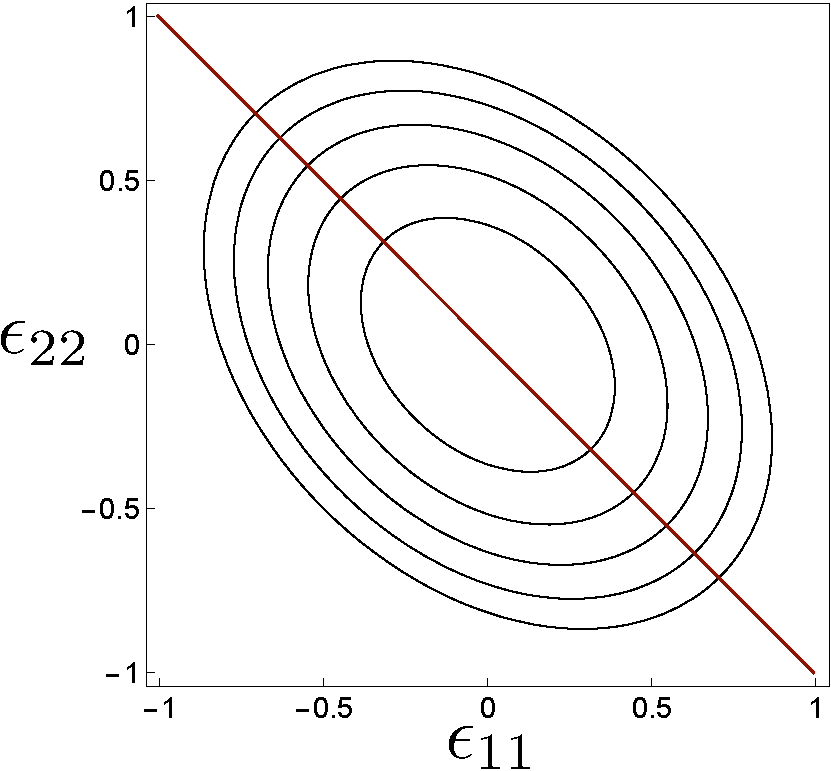
\includegraphics[width=0.3\columnwidth]{ch-fracture/asymmetric_energy/plot_0} &
		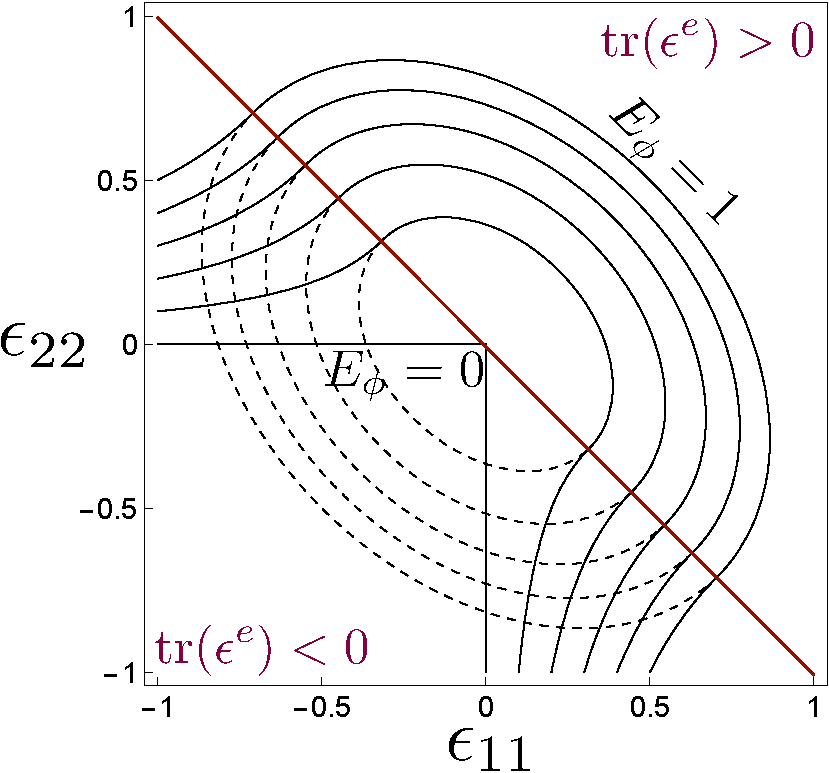
\includegraphics[width=0.3\columnwidth]{ch-fracture/asymmetric_energy/plot_15} &
		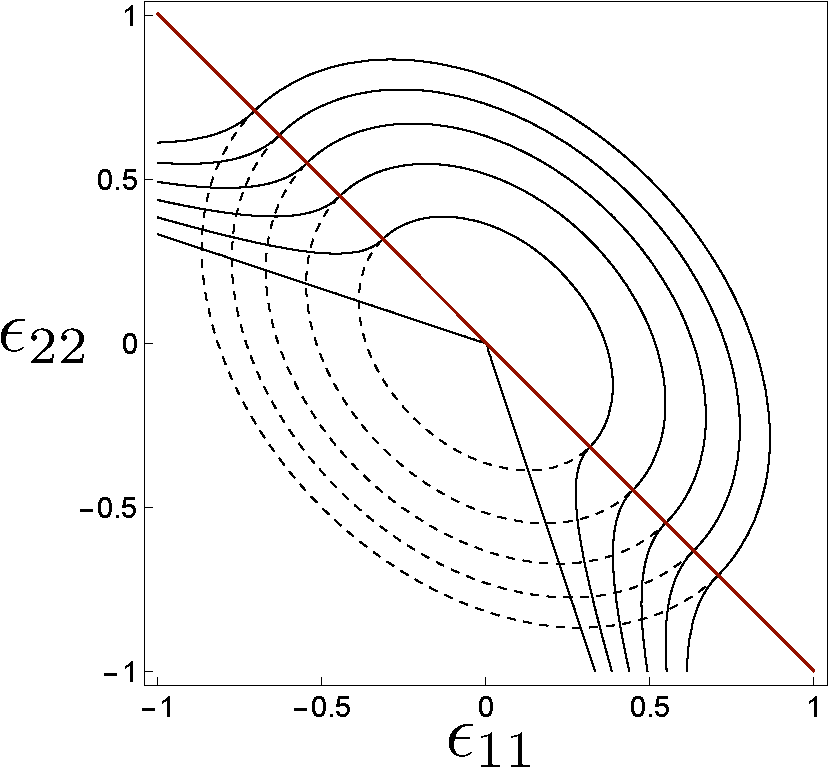
\includegraphics[width=0.3\columnwidth]{ch-fracture/asymmetric_energy/plot_3}  \\
		(a) & (b) & (c)
	\end{tabular}
	\caption{Contours of $E_{\phi}$ with $a=\{0,\tfrac{3}{2},3\}$ are shown in subfigures (a),(b), and (c), respectively. The red, diagonal line indicates the values of strain where $\tr(\eps^e)=0$. Values of $a>1$ break the symmetry between tensile and compressive stresses so that material under local compression is more resistant to fracture.}
	\label{fig:dihedral_angles}
	\end{center}
\end{figure}


\section{Validation}

\subsection{Eshelby's Inclusion Problem}

Eshelby's inclusion problem is used to test that the model and implementation properly resolve the elastic fields resulting from an applied transformation strain. This is a classic problem in micro-mechanics that involves an isolated inclusion embedded within an infinite matrix material. An eigenstrain develops within the constrained inclusion due to phase transformation or thermal expansion and causes stress fields throughout the system. J. D. Eshelby solved for the elastic fields in the interior and exterior of an ellipsoidal inclusion for a given eigenstrain \cite{Eshelby1957, Eshelby1959} . In this section, the results of simulation are compared to his analytical predictions. 



\begin{figure}[h!]
	\begin{center}
	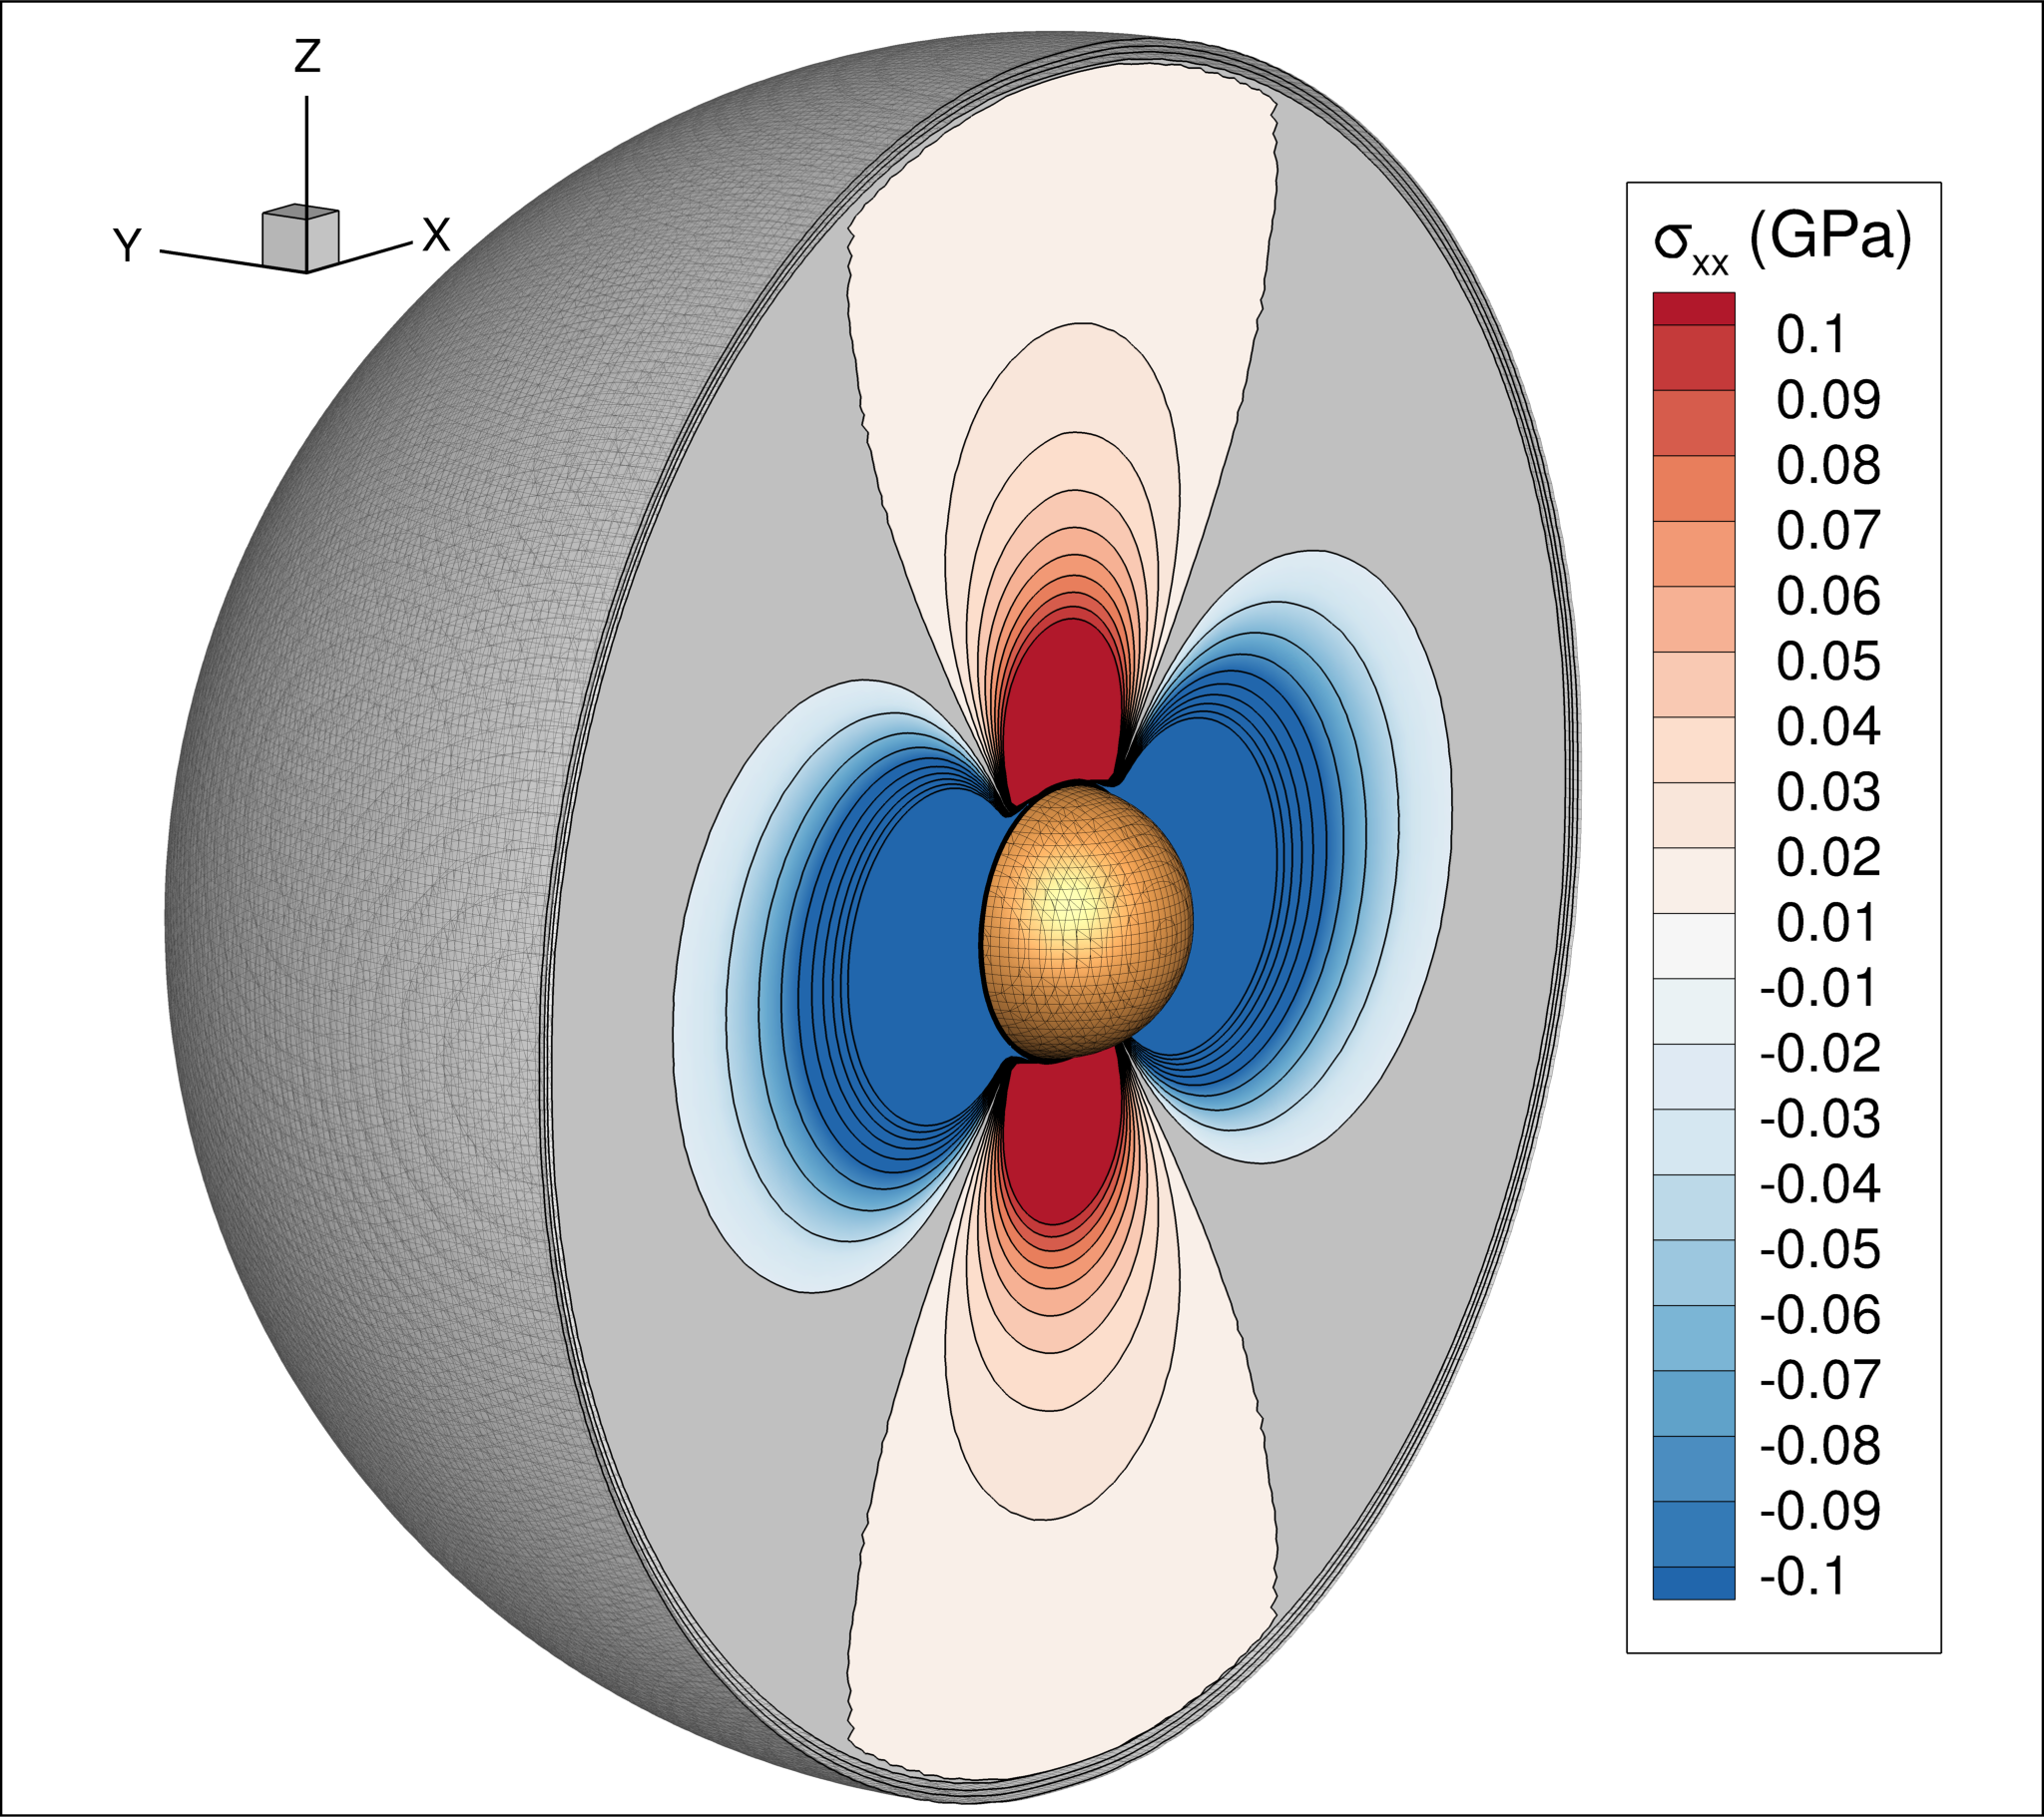
\includegraphics[width=0.6\columnwidth]{ch-fracture/eshelby/inclusion}	
	\caption{The eigenstrain is set to $\eps_T=0.01$ within a spherical inclusion (orange). Contours of the elastic field exterior to the inclusion are plotted within a two-dimensional slice for one component of the stress, $\sigma_{xx}$.}
	\label{fig:eshelby_3d}
	\end{center}
\end{figure}

A test system is configured with a spherical inclusion of radius $a=15$ embedded within the matrix material. Due to the finite limitations of computational simulation, the matrix material will be constrained to a spherical domain that is a factor of six larger in linear size than the inclusion. The system is first coarsened with conserved dynamics to establish a diffuse interface. The materials are set to be elastically homogeneous with Lame's constant and shear modulus given by $\lambda = 150$ and $\mu = 75$ GPa, resulting in $\nu = 1/3$. An eigenstrain, $\eps_T=0.01$, is applied only within the inclusion, and elastic fields are established throughout the system due to this structural inhomogeneity. Figure~\ref{fig:eshelby_3d} shows a three dimensional rendering of the system with a two dimensional slice cutting through the matrix. Contours of one component of the stress tensor, $\sigma_{xx}$, are plotted along the slice and indicate areas of tensile and compressive stress with variations in red and blue color.  

\begin{figure}[h!]
	\begin{center}
	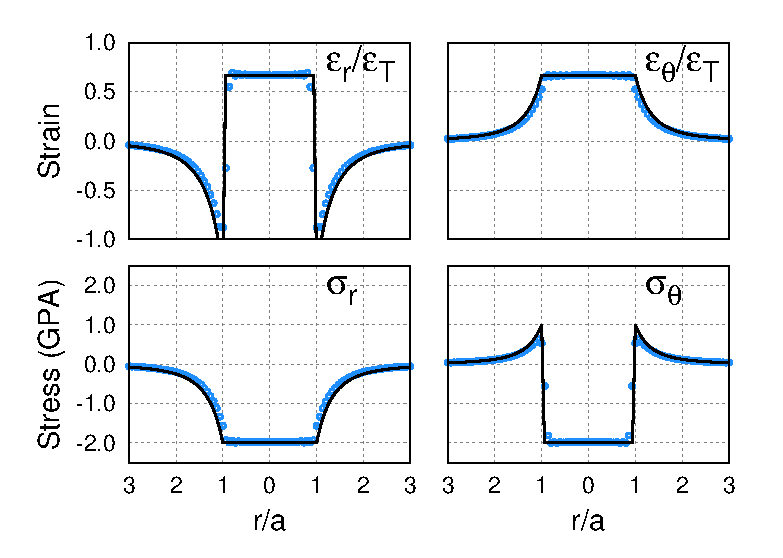
\includegraphics{ch-fracture/eshelby/stress_strain}
	\caption{The subplots display values of the radial and tangential components of the stress and strain against the radial distance from the inclusion's center. The strains are normalized by the eigenstrain in the inclusion, $\eps_T=0.01$. The simulation results (blue symbols) agree closely with analytical predictions (solid black line).}  
	\label{fig:eshelby_results}
	\end{center}
\end{figure}


Insight into the elastic fields that develop as a result of the eigenstrain can be gained through a series of cutting and welding operations envisioned by Eshelby~\cite{Eshelby1957}. If one were to remove the inclusion from the matrix, it would undergo a stress-free strain equal to the eigenstrain. Now, apply a stress that forces the inclusion to its original size and return it to the matrix. An expansion would be observed in the inclusion, but less than that of the eigenstrain. Meanwhile, the matrix would feel compressive strains in the radial direction and tensile strains in the direction tangential to the inclusion surface. Eschelby found that the strain is constant within the inclusion and falls off with the cube of the radial distance within the matrix material. The solutions are summarized in Eq.~\ref{eq:eshelby} \cite{Mura1982}.

\begin{equation}
\begin{alignedat}{2}
	\label{eq:eshelby}
		\eps_r &= \eps_t = \frac{1}{3}\frac{1+\nu}{1-\nu} \eps_T, &&\qquad r<a \\
		\eps_r &= -2\eps_t= \frac{-2}{3} \frac{1+\nu}{1-\nu} \left(\frac{a}{r}\right)^3 \eps_T, &&\qquad r>a
\end{alignedat}
\end{equation}


Figure~\ref{fig:eshelby_results} compares simulation results to the analytical predictions along a line that extends radially from the center of the inclusion and into the matrix. The radial distance is normalize by the inclusion radius, $a=15$ and the strains are normalized by the isotropic eigenstrain within the inclusion, $\eps_T = 0.15$. The data values, shown as blue symbols, agree closely to the analytical predictions, which are plotted as solid black lines. Notice that the strains within the inclusion $r/a<1$ are constant and about 70\% of the applied eigenstrain.

\subsection{Three-Point Bending Test}
 
\section{Results}
\section{Discussion}
%\include{ch-fracture/chapter-fracture}
% \include lets us split up the document (and each include starts a new page):
%\include{ch-intro/chapter-intro}
%\include{ch-conclusion/chapter-conclusion}
%\appendix % all chapters following will be labeled as appendices
%\include{ch-appendicies/implementation}


% Make the bibliography single spaced
\singlespacing
\bibliographystyle{plain}

% add the Bibliography to the Table of Contents
\cleardoublepage
\ifdefined\phantomsection
  \phantomsection  % makes hyperref recognize this section properly for pdf link
\else
\fi
\addcontentsline{toc}{chapter}{Bibliography}

% include your .bib file
\bibliography{thesis}

\end{document}
